
\documentclass[11pt]{article}\usepackage[]{graphicx}\usepackage[]{xcolor}
% maxwidth is the original width if it is less than linewidth
% otherwise use linewidth (to make sure the graphics do not exceed the margin)
\makeatletter
\def\maxwidth{ %
  \ifdim\Gin@nat@width>\linewidth
    \linewidth
  \else
    \Gin@nat@width
  \fi
}
\makeatother

\definecolor{fgcolor}{rgb}{0.345, 0.345, 0.345}
\newcommand{\hlnum}[1]{\textcolor[rgb]{0.686,0.059,0.569}{#1}}%
\newcommand{\hlstr}[1]{\textcolor[rgb]{0.192,0.494,0.8}{#1}}%
\newcommand{\hlcom}[1]{\textcolor[rgb]{0.678,0.584,0.686}{\textit{#1}}}%
\newcommand{\hlopt}[1]{\textcolor[rgb]{0,0,0}{#1}}%
\newcommand{\hlstd}[1]{\textcolor[rgb]{0.345,0.345,0.345}{#1}}%
\newcommand{\hlkwa}[1]{\textcolor[rgb]{0.161,0.373,0.58}{\textbf{#1}}}%
\newcommand{\hlkwb}[1]{\textcolor[rgb]{0.69,0.353,0.396}{#1}}%
\newcommand{\hlkwc}[1]{\textcolor[rgb]{0.333,0.667,0.333}{#1}}%
\newcommand{\hlkwd}[1]{\textcolor[rgb]{0.737,0.353,0.396}{\textbf{#1}}}%
\let\hlipl\hlkwb

\usepackage{framed}
\makeatletter
\newenvironment{kframe}{%
 \def\at@end@of@kframe{}%
 \ifinner\ifhmode%
  \def\at@end@of@kframe{\end{minipage}}%
  \begin{minipage}{\columnwidth}%
 \fi\fi%
 \def\FrameCommand##1{\hskip\@totalleftmargin \hskip-\fboxsep
 \colorbox{shadecolor}{##1}\hskip-\fboxsep
     % There is no \\@totalrightmargin, so:
     \hskip-\linewidth \hskip-\@totalleftmargin \hskip\columnwidth}%
 \MakeFramed {\advance\hsize-\width
   \@totalleftmargin\z@ \linewidth\hsize
   \@setminipage}}%
 {\par\unskip\endMakeFramed%
 \at@end@of@kframe}
\makeatother

\definecolor{shadecolor}{rgb}{.97, .97, .97}
\definecolor{messagecolor}{rgb}{0, 0, 0}
\definecolor{warningcolor}{rgb}{1, 0, 1}
\definecolor{errorcolor}{rgb}{1, 0, 0}
\newenvironment{knitrout}{}{} % an empty environment to be redefined in TeX

\usepackage{alltt}

% Packages for graphics & layout
\usepackage{graphicx}
\usepackage{epstopdf}
\usepackage{caption}
\usepackage{subcaption}
\usepackage{booktabs}
\usepackage[a4paper,margin=0.5in]{geometry}
\usepackage{lipsum}
\usepackage{multicol}

\usepackage[utf8]{inputenc}
\usepackage{enumitem}

% Packages for math
\usepackage{amsmath}
\usepackage{amsfonts}
\usepackage{amssymb}

% Package for bibliography
\usepackage{natbib}
\usepackage{hyperref}

% listing setup \usepackage{listings}
\usepackage{color} % For syntax highlighting color
\captionsetup{labelfont=bf}
\setlength{\parskip}{0.5\baselineskip}


\title{\textbf{Data Analysis Report}}
\author{Michael V Cumbo}
\date{\today}
\IfFileExists{upquote.sty}{\usepackage{upquote}}{}
\begin{document}

\maketitle

\section{Introduction}
This paper was written in response to the United Auto Workers strike and the SAG-AFTRA strike of 2023. The goal of gathering the data is to contextualize the state of trade union power in the United States, blending data analysis with a literature review. 
The data in this paper will contextualize union power in a select number of nation-states, adding perspective to the modes of influence unions have.

This report is a month to month analysis of labor action tracker newly recorded data. The report should give an assessment of trends in the strike activity.
The regions in focus will be the DMV which consist of The District of Columbia, Maryland and Virginia.

\section{Data Prep}
\begin{knitrout}
\definecolor{shadecolor}{rgb}{0.969, 0.969, 0.969}\color{fgcolor}\begin{kframe}
\begin{alltt}
\hlkwd{source}\hlstd{(}\hlstr{"~/Lab2/Trade_Union_Global_Analysis/summary_analysis/Enviroment_Setup.R"}\hlstd{)}

\hlkwd{suppressPackageStartupMessages}\hlstd{(\{}
  \hlkwd{library}\hlstd{(ggplot2)}
  \hlkwd{library}\hlstd{(dplyr)}
\hlstd{\})}

\hlcom{# connect to the database and pull out the sheet}
\hlkwd{setwd}\hlstd{(}\hlstr{"~/workbook"}\hlstd{)}
\hlstd{con} \hlkwb{<-} \hlkwd{dbConnect}\hlstd{(RSQLite}\hlopt{::}\hlkwd{SQLite}\hlstd{(),} \hlstr{"trade_union_data.db"}\hlstd{)}
\hlkwd{dbListTables}\hlstd{(con)}
\end{alltt}
\begin{verbatim}
##  [1] "CBCR"                                    
##  [2] "CollectiveBargaining"                    
##  [3] "ILRLaborActionTracker"                   
##  [4] "IRL&ScrappedDataComparision"             
##  [5] "LAT-02.19.24"                            
##  [6] "LAT-03.04.24"                            
##  [7] "LAT-04.01.24"                            
##  [8] "State_Union_Coverage_Density_1977-2021"  
##  [9] "State_Union_Membership_Density_1964-2021"
## [10] "Strikes_United_States"                   
## [11] "TUDR"                                    
## [12] "TradeUnionDensity"                       
## [13] "WorkplaceRights"                         
## [14] "raw_strike_table"                        
## [15] "rawonlystrike_table"                     
## [16] "state_union_coverage_density_long"       
## [17] "state_union_membership_density_long"     
## [18] "state_uniondc_join"                      
## [19] "strike_table"                            
## [20] "summarytable_IRLvSData"
\end{verbatim}
\begin{alltt}
\hlstd{february} \hlkwb{<-} \hlkwd{as_tibble}\hlstd{(}\hlkwd{dbReadTable}\hlstd{(con,} \hlstr{"LAT-02.19.24"}\hlstd{))}
\hlkwd{dbDisconnect}\hlstd{(con)}
\end{alltt}
\end{kframe}
\end{knitrout}

\begin{knitrout}
\definecolor{shadecolor}{rgb}{0.969, 0.969, 0.969}\color{fgcolor}\begin{kframe}
\begin{alltt}
\hlcom{# Convert Timestamp column to POSIXct format}
\hlstd{february}\hlopt{$}\hlstd{Timestamp} \hlkwb{<-} \hlkwd{as.POSIXct}\hlstd{(february}\hlopt{$}\hlstd{Timestamp,}
  \hlkwc{format} \hlstd{=} \hlstr{"%m/%d/%Y %H:%M:%S"}
\hlstd{)}

\hlcom{# mutate zip code to a character}
\hlstd{february} \hlkwb{<-} \hlstd{february} \hlopt
  \hlkwd{mutate}\hlstd{(}
    \hlkwc{ZipCode} \hlstd{=} \hlkwd{as.character}\hlstd{(ZipCode),}
    \hlkwc{BargainingUnitSize} \hlstd{=} \hlkwd{parse_number}\hlstd{(}\hlkwd{as.character}\hlstd{(BargainingUnitSize)),}
    \hlkwc{ApproximateNumberofParticipants} \hlstd{=}
      \hlkwd{parse_number}\hlstd{(}\hlkwd{as.character}\hlstd{(ApproximateNumberofParticipants)),}
    \hlkwc{Date} \hlstd{=} \hlkwd{format}\hlstd{(Timestamp,} \hlstr{"%Y-%m-%d"}\hlstd{),}
    \hlkwc{month} \hlstd{=} \hlkwd{format}\hlstd{(Timestamp,} \hlstr{"%B"}\hlstd{),}
    \hlkwc{Year} \hlstd{=} \hlkwd{format}\hlstd{(Timestamp,} \hlstr{"%Y"}\hlstd{),}
    \hlkwc{DurationAmount} \hlstd{=} \hlkwd{as.integer}\hlstd{(DurationAmount)}
  \hlstd{)}
\end{alltt}
\end{kframe}
\end{knitrout}

\begin{knitrout}
\definecolor{shadecolor}{rgb}{0.969, 0.969, 0.969}\color{fgcolor}\begin{kframe}
\begin{verbatim}
## [1] "the total number of available data points in the BargainingUnitSize vector is 211"
## [1] "the total number of missing/blank data points in the BargainingUnitSize vector is 2655"
## [1] "the total number of missing/blank data points in the notes vector is 380"
\end{verbatim}
\end{kframe}
\end{knitrout}




\clearpage
\section{Data Analysis}


\begin{knitrout}
\definecolor{shadecolor}{rgb}{0.969, 0.969, 0.969}\color{fgcolor}

{\centering 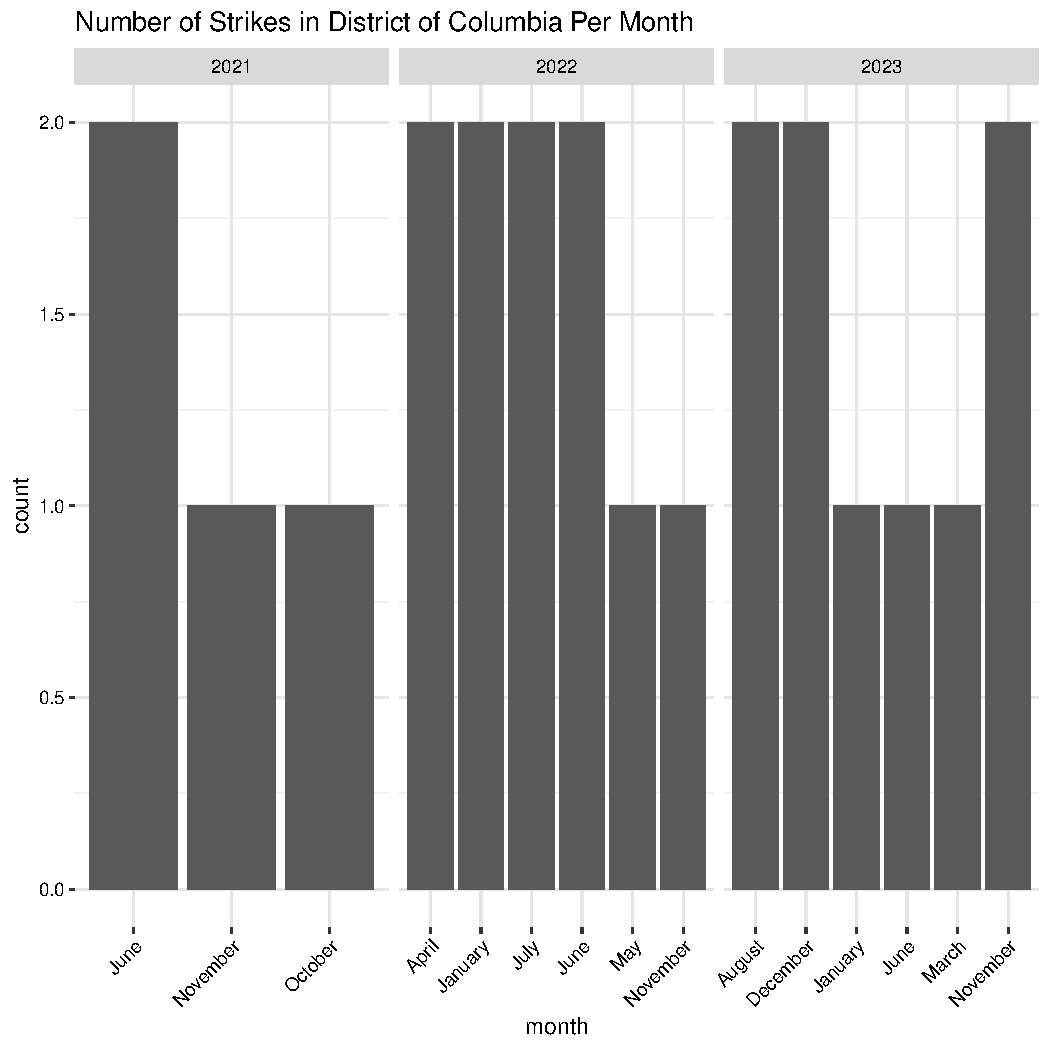
\includegraphics[width=0.7\linewidth]{figure/calling_the_ggplots_for_DC-1} 

}


\begin{kframe}\begin{verbatim}
## The number of active labor organizations during the selected 
##  period of 2021, 2022, 2023, 2024 in District of Columbia is 18 .
## # A tibble: 3 x 4
##   State                Year  labor_org_count strikes
##   <chr>                <chr>           <int>   <int>
## 1 District of Columbia 2021                3       4
## 2 District of Columbia 2022                7      10
## 3 District of Columbia 2023                8       9
\end{verbatim}
\end{kframe}
\end{knitrout}

\begin{knitrout}
\definecolor{shadecolor}{rgb}{0.969, 0.969, 0.969}\color{fgcolor}

{\centering 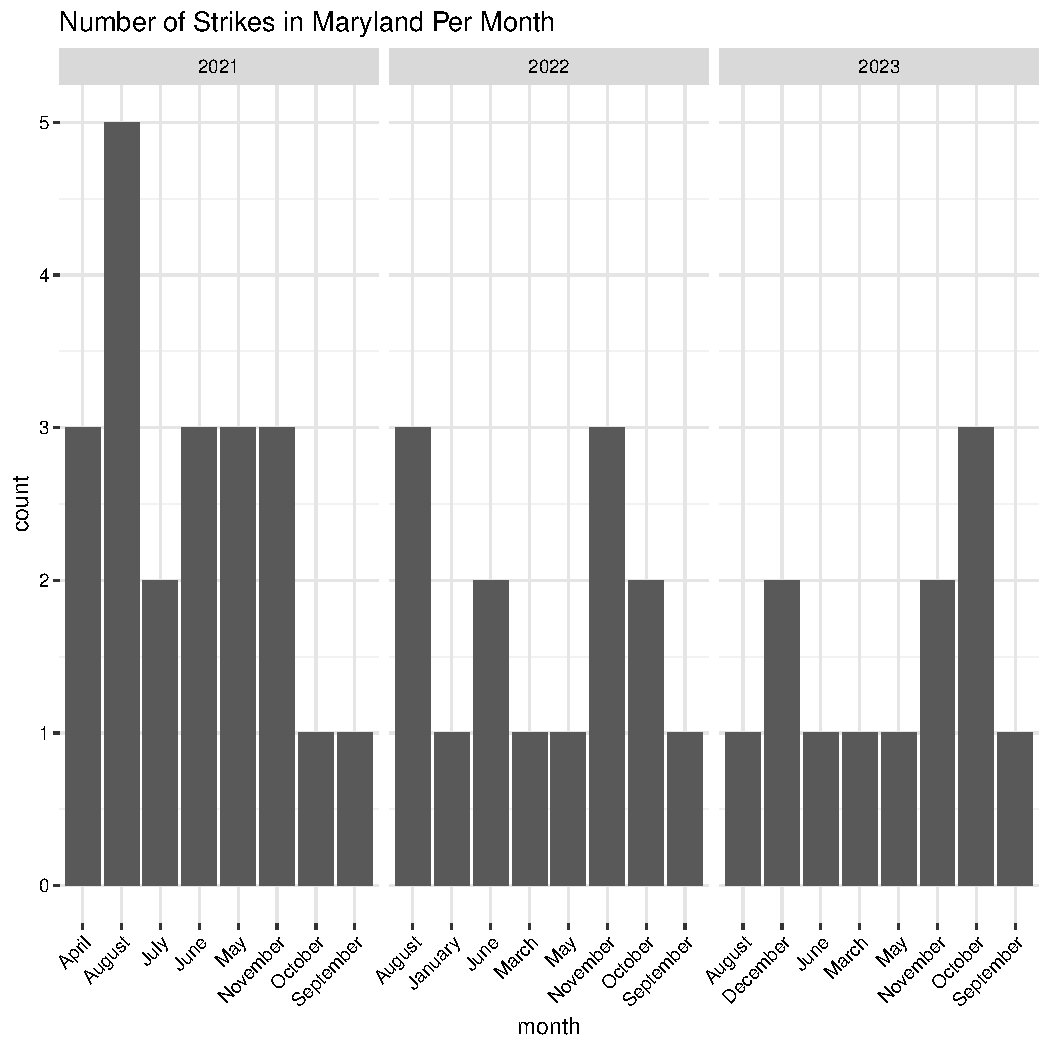
\includegraphics[width=0.7\linewidth]{figure/calling_the_ggplots_for_Maryland-1} 

}


\begin{kframe}\begin{verbatim}
## The number of active labor organizations during the selected 
##  period of 2021, 2022, 2023, 2024 in Maryland is 36 .
## # A tibble: 3 x 4
##   State    Year  labor_org_count strikes
##   <chr>    <chr>           <int>   <int>
## 1 Maryland 2021               11      21
## 2 Maryland 2022               14      14
## 3 Maryland 2023               11      12
\end{verbatim}
\end{kframe}
\end{knitrout}

\begin{knitrout}
\definecolor{shadecolor}{rgb}{0.969, 0.969, 0.969}\color{fgcolor}

{\centering 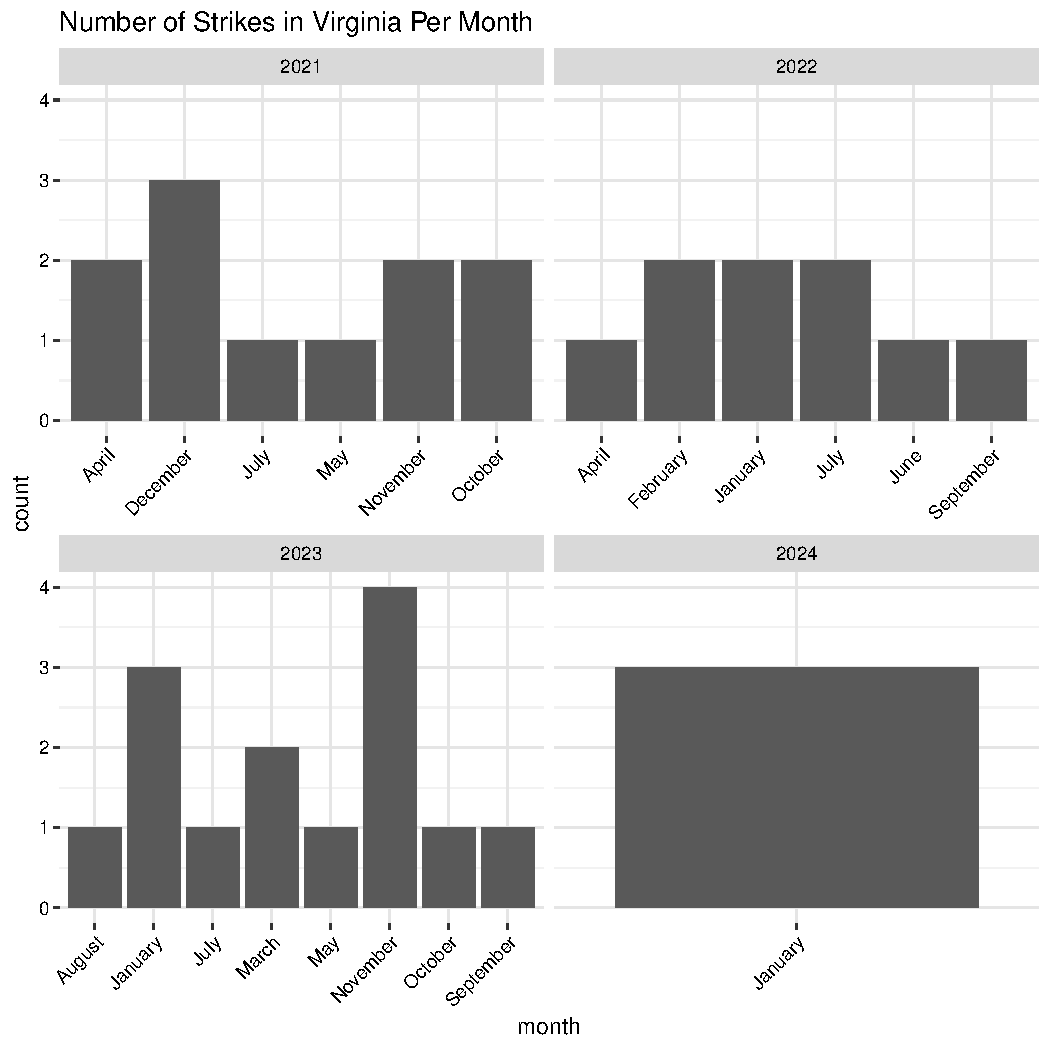
\includegraphics[width=0.7\linewidth]{figure/calling_the_ggplots_Virginia-1} 

}


\begin{kframe}\begin{verbatim}
## The number of active labor organizations during the selected 
##  period of 2021, 2022, 2023, 2024 in Virginia is 28 .
## # A tibble: 4 x 4
##   State    Year  labor_org_count strikes
##   <chr>    <chr>           <int>   <int>
## 1 Virginia 2021                8      11
## 2 Virginia 2022                7       9
## 3 Virginia 2023               12      14
## 4 Virginia 2024                1       3
\end{verbatim}
\end{kframe}
\end{knitrout}

\end{document}
